\chapter{Taler}

\section{Taler Architecture}

\subsection{Auditor}
The following text is cited from section 4.4 in \cite{dold:the-gnu-taler-system}
\begin{center}
    \textit{
        "The auditor consists of two processes that are regularly run and generate auditing reports.  
        Both processes access the exchange’s database, either directly (for exchange-internal auditing as part if its operational security) or over a replica (in the case of external auditors).
        The taler-wire-auditor process checks that the incoming and outgoing transfers recorded in the exchange’s database match wire transfers of the underlying  bank  account.   
        To access the transaction history (typically recorded by the bank), the wire auditor uses a wire plugin, with the same interface and implementation as the exchange’s wire plugins.
        The taler-auditor process generates a report with the following information:
    }
\end{center}

\begin{itemize}
    \item \textit{Do the operations stored in a reserve’s history match the reserve’s balance?}
    \item \textit{Did the exchange record outgoing transactions to the right merchant for deposits after the deadline for the payment was reached?}
    \item \textit{Do operations recorded on coins (deposit, refresh, refund) match the remaining value on the coin?}
    \item \textit{Do operations respect the expiration of denominations?}
    \item \textit{For a denomination, is the number of pairwise different coin public keys recorded in deposit/refresh operations smaller or equal to the number of blind signatures recorded in withdraw/refresh operations? If this invariant is violated, the corresponding denomination must be revoked.}
    \item \textit{What is the income if the exchange from different fees?}
\end{itemize}

\begin{center}
    \textit{
        \dots
        The auditor exposes a web server with the taler-auditor-httpd process.
        Currently, it only shows a website that allows the customer to add the auditor to the list of trusted auditors in their wallet. 
        In future versions, the auditor will also have HTTP endpoints that allow merchants to submit samples of deposit confirmations,  which  will  be  checked  against  the  deposit  permissions  in  the exchange’s  database  to  detect  compromised  signing  keys  or  missing  writes.
        Furthermore,  in  deployments  that  require  the  merchant  to  register  with  the exchange beforehand, the auditor also offers a list of exchanges it audits, so that the merchant backend can automatically register with all exchanges it transitively trusts."
    }
\end{center}
Some details were left out (see at the dots) and can be read in section 4.4 in \cite{dold:the-gnu-taler-system}

\subsubsection{Technical Details}
Documentation: \cite{taler-documentation:auditor-operator-manual} \\
Git Repositories:
\begin{itemize}
    \item Main repository: \cite{taler-git:exchange} (Part of exchange repository, inside ./src/auditor and ./src/auditordb)
    \item Auditor's public website: \cite{taler-git:auditor}
\end{itemize}
Language: C \\
Dependencies: 
\begin{itemize}
    \item GNUnet            >= 0.14.0
    \item GNU libmicrohttpd >= 0.9.71
    \item Postgres          >= 9.6, including libpq
    \item libjansson        >= 2.7
    \item libargon2         >= 20171227
    \item libsodium         >= 1.0
    \item libgcrypt         >= 1.6
    \item libqrencode       >= 4.0.0
    \item libcurl           >= 7.26 (or libgnurl >= 7.26)
    \item GNU libunistring  >= 0.9.3
    \item libsqlite3        >= 3.16.2
\end{itemize}
The auditor API is implemented as REST API and uses \ac{JSON} as message format.
The auditor does not implement HTTPS (TLS), instead it recommends using a HTTP reverse Proxy that offers TLS termination.
By delegating the responsibility for TLS termination, the auditor implementation becomes lighter.

There are a lot more technical details written in the documentation linked above and in the README files.
Since Taler is actively developed and technical details could change, we refer to this documentation.

\subsection{Exchange}
The following text is cited from section 4.3 in \cite{dold:the-gnu-taler-system}
\begin{center}
    \textit{
        "The exchange consists of three independent processes:
    }
\end{center}
\begin{itemize}
    \item \textit{The taler-exchange-httpd process handles HTTP requests from clients, mainly merchants and wallets.}
    \item \textit{The taler-exchange-wirewatch process watches for wire transfers to the exchange’s bank account and updates reserves based on that.}
    \item \textit{The taler-exchange-aggregator process aggregates outgoing transactions to merchants.}
\end{itemize}

\begin{center}
    \textit{
        All three processes exchange data via the same database. 
        Only taler-exchange-httpd needs access to the exchanges online signing keys and denomination keys.
        The database is accessed via a Taler-specific database abstraction layer. 
        Different databases  can  be  supported  via  plugins;  at  the  time  of  writing  this,  only  a PostgreSQL plugin has been implemented.
        Wire plugins are used as an abstraction to access the account layer that Taler runs on. 
        Specifically, the wirewatch process uses the plugin to monitor incoming transfers, and the aggregator process uses the wire plugin to make wire transfers to merchants.
        The following APIs are offered by the exchange:
    }

    \textbf{\textit{Announcing keys, bank accounts and other public information}}\\
    \textit{
            The exchange offers the list of denomination keys, signing keys, auditors, supported bank accounts, revoked keys and other general information needed to use the exchange’s services via the /keys and /wire APIs.
    }

    \textbf{\textit{Reserve status and withdrawal}}\\
    \textit{
            After having wired money to the exchange, the status of the reserve can be checked via the /reserve/status API. Since the wire transfer usually takes some time to arrive at the exchange, wallets should periodically poll this API, and initiate a withdrawal with /reserve/withdraw once the exchange received the funds.
    }

    \textbf{\textit{Deposits and tracking}}\\
    \textit{
            Merchants transmit deposit permissions they have received from customers to the exchange via the/deposit API. Since multiple deposits are aggregated into one wire transfer, the merchant additionally can use the exchange’s /track/transfer API that returns the list of deposits for an identifier included in the wire transfer to the merchant, as well as the /track/transaction API to look up which wire transfer included the payment for a given deposit.
    }

    \textbf{\textit{Refunds}}\\
    \textit{
            The refund API (/refund) can “undo” a deposit if the merchant gave their signature, and the aggregation deadline for the payment has not occurred yet.    
    }

    \textbf{\textit{Emergency payback}}\\
    \textit{
            The emergency payback API (/payback) allows customers to be compensated for coins whose denomination key has been revoked.
            Customers must send either a full withdrawal transcript that includes their private blinding factor, or a refresh transcript (of a refresh that had the revoked denominations as one of the targets) that includes blinding factors.
            In the former case, the reserve is credited, in the latter case, the source coin of the refresh is refunded and can be refreshed again."
    }
\end{center}

Additional information for how the exchange generates new denomination and signing keys can be found in the end of section 4.3 of \cite{dold:the-gnu-taler-system}.

\begin{figure}[h!]
    \centering
    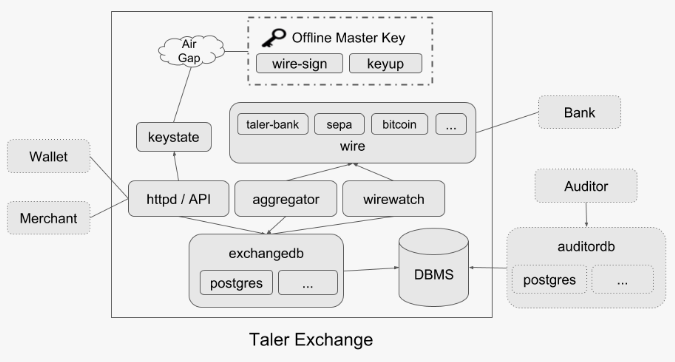
\includegraphics[height=0.5\textwidth]{taler-exchange.png}
    \caption{Architecture of the Taler Exchange reference implementation. Source: \cite{dold:the-gnu-taler-system}}
    \label{fig:taler-arch-exchange}
\end{figure}

\subsubsection{Technical Details}

Documentation: \cite{taler-documentation:exchange-operator-manual} \\
Git Repository: Main repository: \cite{taler-git:exchange} \\
Language: C \\
Dependencies: 
\begin{itemize}
    \item GNUnet            >= 0.14.0
    \item GNU libmicrohttpd >= 0.9.71
    \item Postgres          >= 9.6, including libpq
    \item libjansson        >= 2.7
    \item libargon2         >= 20171227
    \item libsodium         >= 1.0
    \item libgcrypt         >= 1.6
    \item libqrencode       >= 4.0.0
    \item libcurl           >= 7.26 (or libgnurl >= 7.26)
    \item GNU libunistring  >= 0.9.3
    \item libsqlite3        >= 3.16.2
\end{itemize}
The exchange’s API is implemented as REST API and uses \ac{JSON} as message format.

There are a lot more technical details written in the documentation linked above and in the README files.
Since Taler is actively developed and technical details could change, we refer to this documentation.

\subsection{Merchant}
The following text is cited from section 4.5 in \cite{dold:the-gnu-taler-system}
\begin{center}
    \textit{
        "The Taler merchant backend is a component that abstracts away the details of processing Taler payments and provides a simple HTTP API.
        The merchant backend handles cryptographic operations (signature verification, signing), secret management and communication with the exchange.
        The backend API (see \url{https://docs.taler.net/api/}) is divided into two types of HTTP endpoints:
    }
\end{center}

\begin{enumerate}
    \item \textit{Functionality that is accessed internally by the merchant. 
    These API stypically require authentication and/or are only accessible from within the private network of the merchant.}
    \item \textit{Functionality that is exposed publicly on the Internet and accessed by the customer’s wallet and browser.}
\end{enumerate}

\begin{center}
    \textit{
        A typical merchant has a storefront component that customers visit with their browser, as well as a back office component that allows the merchant to view information about payments that customers made and that integrates with other components such as order processing and shipping."
    }
\end{center}

\subsubsection{Processing Payments}
\begin{center}
    \textit{
        "To process a payment, the storefront first instructs the backend to create an order.
        The order contains information relevant to the purchase, and is in fact a subset of the information contained in the contract terms. 
        The backend automatically adds missing information to the order details provided by the storefront. 
        The full contract terms can only be signed once the customer provides the claim public key for the contract.\\
        Each order is uniquely identified by an order ID, which can be chosen by the storefront or automatically generated by the backend.
        The order ID can be used to query the status of the payment. 
        If the customer did not pay for an order ID yet, the response from the backend includes a payment redirect URL.
        The storefront can redirect the customer to this payment redirect URL; visiting the URL will trigger the customer’s browser/wallet to prompt for a payment.\\
        To simplify the implementation of the storefront, the merchant backend can serve a page to the customer’s browser that triggers the payment via the HTTP402 status code and the corresponding headers, and provides a fallback (in the form of a taler:pay link) for loosely integrated browsers. 
        When checking the status of a payment that is not settled yet, the response from the merchant backend will contains a payment redirect URL. 
        The storefront redirects the browser to this URL, which is served by the merchant backend and triggers the payment.
        \dots "
    }
\end{center}

\subsubsection{Back Office APIs}
\begin{center}
    \textit{
        "The back office API allows the merchant to query information about the history and status of payments, as well as correlate wire transfers to the merchant’s bank account with the respective GNU Taler payment. 
        This API is necessary to allow integration with other parts of the merchant’s e-commerce infrastructure."
    }
\end{center}

% Nachfolgende Section nicht notwendig.
% \subsubsection{Example Merchant Frontends}
% This section is included to provide an overview of the reference implementation for the merchant.
% This helps to get a better understanding of how a merchant could potentially look like.
% Note that the actual code could differ from the cited part.
% The actual code can be found in \url{git.taler.net}
% \begin{center}
%     \textit{
%         We implemented the following applications using the merchant backend API.
%     }
    
%     \textit{\textbf{Blog Merchant}}\\
%     \textit{
%         The blog merchant’s landing page has a list of article titles with a teaser. 
%         When following the link to the article, the customer is asked to pay to view the article.
%     }

%     \textit{\textbf{Donations}}\\
%     \textit{
%         The donations frontend allows the customer to select a project to donate to.
%         The fulfillment page shows a donation receipt.
%     }

%     \textit{\textbf{Codeless Payments}}\\
%     \textit{
%         The codeless payment frontend is a prototype for a user interface that allows merchants to sell products on their website without having to write code to integrate with the merchant backend.
%         Instead, the merchant uses a web interface to manage products and their available stock.
%         The codeless payment frontend then creates an HTML snippet with a payment button that the merchant can copy-and-paste integrate into their storefront.
%     }

%     \textit{\textbf{Survey}}\\
%     \textit{
%         The survey frontend showcases the tipping functionality of GNU Taler.
%         The user fills out a survey and receives a tip for completing it.
%     }

%     \textit{\textbf{Back Office}}\\
%     \textit{
%         The example back-office application shows the history and status of payments processed by the merchant.
%     }
% \end{center}

\begin{figure}[h!]
    \centering
    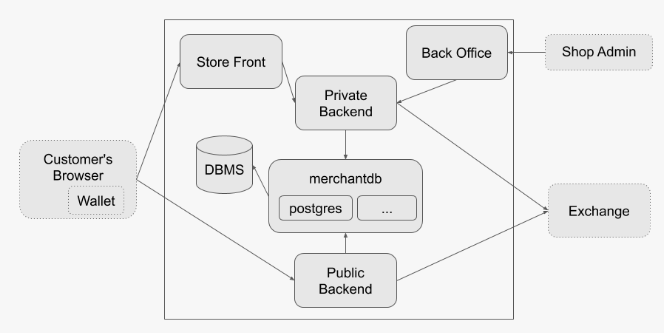
\includegraphics[height=0.5\textwidth]{taler-merchant.png}
    \caption{Architecture Taler Merchant reference implementation. Source: \cite{dold:the-gnu-taler-system}}
    \label{fig:taler-arch-merchant}
\end{figure}

\subsubsection{Technical Details}

Documentation: \cite{taler-documentation:merchant-backend-operator-manual} \\
API Documentation: \cite{taler-documentation:merchant-api} \\
Back-office Documentation: \cite{taler-documentation:back-office} \\
Point-of-Sales Documentation: \cite{taler-documentation:pos-manual} \\
Git Repositories: 
\begin{itemize}
\item Backend: \cite{taler-git:merchant}
\item Backoffice: \cite{taler-git:backoffice}
\item Point-of-Sales App: \cite{taler-git:android} (part of android repo)
\end{itemize}
Language: C (Backend), Kotlin (\ac{PoS}), [Python, Javascript] (Backoffice)\\
Dependencies: 
\begin{itemize}
    \item GNUnet            >= 0.14.0
    \item GNU libmicrohttpd >= 0.9.71
    \item Postgres          >= 9.6, including libpq
    \item libjansson        >= 2.7
    \item libargon2         >= 20171227
    \item libsodium         >= 1.0
    \item libgcrypt         >= 1.6
    \item libqrencode       >= 4.0.0
    \item libcurl           >= 7.26 (or libgnurl >= 7.26)
    \item GNU libunistring  >= 0.9.3
    \item libsqlite3        >= 3.16.2
    \item Flask (Backoffice)
\end{itemize}
Frontend Repositories:
\begin{itemize}
    \item Payments with Django: \cite{taler-git:django-payments}
    \item Wordpress woocommerce plugin: \cite{taler-git:woocommerce}
    \item Saleor Frontend: \cite{taler-git:saleor}
    \item Demo Frontends: \cite{taler-git:merchant-demos}
\end{itemize}
The merchant’s API is implemented as REST API and uses \ac{JSON} as message format.
The \ac{PoS} app is for the merchant to process customer's orders by adding or removing products, calculating the amount owed by the customer or letting the customer make a Taler payment via QR code or NFC.
The back office Web service allows a merchant to check status of their Taler transactions.
There are already a lot of demo pages and integrations for different e-commerce solutions.

There are a lot more technical details written in the documentation linked above and in the README files.
Since Taler is actively developed and technical details could change, we refer to this documentation.

\subsection{Wallet}
The following text is cited from section 4.6 in \cite{dold:the-gnu-taler-system}
\begin{center}
    \textit{
        "The wallet manages the customer’s reserves and coins, lets the customer view and pay for contracts from merchants. \dots
        The reference implementation of the GNU Taler wallet is written in the Type-Script language against the WebExtension API, a cross-browser mechanism for browser extensions.
        The reference wallet is a “tightly integrated” wallet, as it directly hooks into the browser to process responses with the HTTP status code“402 Payment Required”.\\
        Many cryptographic operations needed to implement the wallet are not commonly available in a browser environment.
        We cross-compile the GNU Taler utility library written in C as well as its dependencies (such as libgcrypt) to asm.js (and WebAssembly on supported platforms) using the LLVM-based emscripten toolchain.
        Cryptographic operations run in an isolated process implemented as a WebWorker.
        This design allows the relatively slow cryptographic operations to run concurrently in the background in multiple threads.
        Since the crypto WebWorkers are started on-demand, the wallet only uses minimal resources when not actively used."
    }
\end{center}

\subsubsection{Optimizations}
\begin{center}
    \textit{
        "To improve the perceived performance of cryptographic operations, the wallet optimistically creates signatures in the background while the user is looking at the “confirm payment” dialog.
        If the user does not accept the contract, these signatures are thrown away instead of being sent to the merchant.
        This effectively hides the latency of the most expensive cryptographic operations, as they are done while the user consciously needs to make a decision on whether to proceed with a payment."
    }
\end{center}

\subsubsection{Wallet Detection}
\begin{center}
    \textit{
        " \dots
        Browser fingerprinting is a concern with any additional APIs made available to websites, either by the browser itself or by browser extensions.
        Since a website can simply try to trigger a payment to determine whether a tightly integrated Taler wallet is installed, one bit of additional fingerprinting information is already available through the usage of Taler.
        The dynamic detection methods do not, however, expose any information that is not already available to websites by signaling the wallet through HTTP headers."
    }
\end{center}

\subsubsection{Further Wallet Features}
More information about other Wallet Features like coin selection, wallet liquidation and wallet signaling can be found in sections 4.6.2, 4.6.5 and 4.6.6 of \cite{dold:the-gnu-taler-system}.

\begin{figure}[h!]
    \centering
    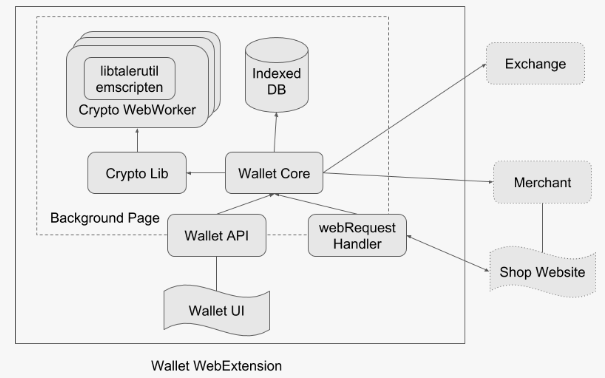
\includegraphics[height=0.5\textwidth]{taler-wallet.png}
    \caption{Architecture of the Taler Wallet reference implementation. Source: \cite{dold:the-gnu-taler-system}}
    \label{fig:taler-wallet-reference-impl}
\end{figure}

\subsubsection{Technical Details}

Documentation: \cite{taler-documentation:wallet-developer-manual} \\
Wallet-CLI documentation: \cite{taler-documentation:wallet-cli-manual} \\
Git Repository: 
\begin{itemize}
    \item Main repository: \cite{taler-git:wallet-core} \\
    This Repository includes the wallet-core and the implementations for the web extension and CLI.
    \item Android app: \cite{taler-git:android}
    \item iOS app: \cite{taler-git:ios}
\end{itemize}
Language: Typescript, Javascript (wallet-core,  web extension), Kotlin (Android app), Swift (iOS app)\\
Dependencies: 
\begin{itemize}
    \item prettier            
    \item rimraf
    \item rollup
    \item typescript
    \item ava
    \item esbuild
    \item axios
    \item tslib
    \item cancellationtoken
    \item minimatch
    \item source-map-support
    \item big-integer
    \item fflate
    \item esm
    \item jed
    \item nyc
    \item po2json
    \item typedoc
    \item api-extractor
\end{itemize}

There are a lot more technical details written in the documentation linked above and in the README files.
Since Taler is actively developed and technical details could change, we refer to this documentation.


